
\section{Results from the multivariate analysis}
\label{sec:mva}

From the cut-based analysis,
combining the significance of the three categories,
we end up with a signal significance of $S/\sqrt{B}\simeq 1.2(2.3)$
with all backgrounds (only QCD $4b$) taken into account.
%
This does not seem
to be enough to be able to claim observation
of Higgs pair production
in this channel, and even less to extract the trilinear Higgs  coupling
$\lambda$ with good precision.
%
In this section we show how the signal significance for
our process can
be substantially improved when
applying a multivariate analysis (MVA) to the events
 that survive the cut-based
 analysis.

 
%
Multivariate techniques are by now a common tool to enhance signal
significance in HEP analysis, and this is fully justified
since they open a new window to improve the performance
of many physics analysis and searches.
%
In particular, the classification of events as arising from either signal or
background processes via the use of a multivariate analysis is becoming
a mature
technique in LHC
applications~\cite{Baldi:2014pta,Aaltonen:2012qt,
  Wardrope:2014kya,Chatrchyan:2013zna,Dall'Osso:2015aia}.
%
For instance, the CMS $Vh(\to b\bar{b})$ analysis~\cite{Chatrchyan:2013zna}
is based on a Boosted Decision Tree (BDT) MVA, and the UCL $hh\to 4b$
feasibility study~\cite{Wardrope:2014kya}
also used  a BDT to improve signal discrimination.

In this section, first of all we present the specific MVA that we use,
based on feed-forward multi-layer neural networks.
%
We then introduce the input variables that are
used the MVA, including the jet substructure
variables, and then present the results of $S/\sqrt{B}$ including
the MVA effects.
%
Since we find that jet substructure variables are a crucial input
to the MVA, we end this section showing various kinematic distributions
of these variables.



\subsection{MVA strategy: deep neural networks}


%
In our work we use a specific type of  MVA to
disentangle signal and background events in the $hh\to 4b$ process,
a multi-layer feed-forward artificial neural network (ANN),
also known as a {\it perceptron}.\footnote{This type of ANNs are the same
  as those used to parametrize Parton Distribution Functions
in the NNPDF global analyses~\cite{DelDebbio:2004qj,Ball:2008by,Ball:2011mu,Ball:2010de}.}
%
This family of ANNs is sometimes known as {\it deep} neural networks.
%
The basic idea is that the ANN is trained on an input composed on
all  signal and background
events which satisfy the requirements of the
cut-based analysis.
%
The main result of the trained ANN is identifying, in a fully automated way,
which are the most relevant variables to discriminate between the two.

In this work, the ANN that we use has the following architecture.
\be
\label{eq:nn1}
N_{\mathrm{var}}\times5\times3\times1 \, ,
\ee
where $N_{\mathrm{var}}$ represents the number of input variables for the MVA.
All neural-network layers use a sigmoid activation function, allowing
for a probabilistic
interpretation of the neural-network output, including in the final layer.
%
In Fig.~\ref{fig:nnarch} we show an example of the ANN that we use in this work, corresponding here
to the case of the resolved category.

%%%%%%%%%%%%%%%%%%%%%%%%
\begin{figure}[t]
  \begin{center}
      \vspace{-1cm}
  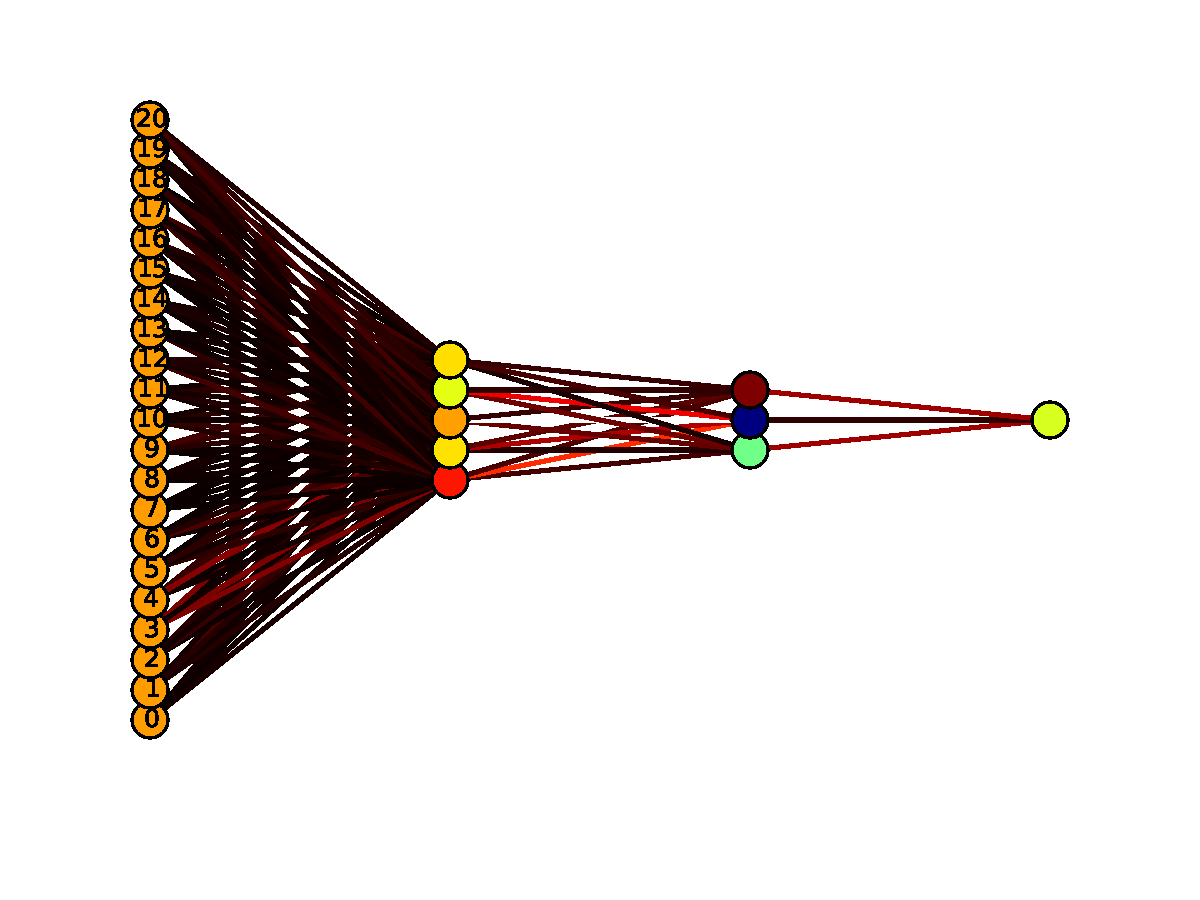
\includegraphics[width=0.90\textwidth]{plots/bst_nnarch_noPU.pdf}
  \vspace{-1cm}
  \caption{\small Architecture of the ANN used for the analysis of the
    boosted
    category, with $N_{\rm var}=21$ input variables and thus
    the same number of neurons
  in the first layer.
  %
  The color code in the neuron connections (the weights) is a heat map,
  with red indicating large values and black small values.
}
\label{fig:nnarch}
\end{center}
\end{figure}
%%%%%%%%%%%%%%%%%%%%%%%

The training of the ANN for the signal/background classification task
proceeds as follows.
%
Given a set of $N_{\mathrm{var}}$  kinematic variables $\{k\}_i$ associated with the event $i$, and a set of neural network parameters $\{\omega\}$, we interpret the neural network output $y_i$ (that is, the activation state of the
neuron in the last layer)
as the probability that the event $i$ originates from the signal process,
\be
y_i = P(y^\prime_i=1|\{k\}_i, \{\omega\} )\, ,
\ee
where $y_i^\prime$ represents the true classification of the event $i$, i.e $y^\prime_{\text{signal}} = 1$ and $y^\prime_{\text{background}} = 0$. With this interpretation, our general classification probability including background events is given by
\be
P(y_i^\prime|\{k\}_i, \{\omega\}) = y_i^{y^\prime_i}(1-y_i)^{1-y^\prime_i} \, ,
\ee
which implies that the  negative log-likelihood cost function
that needs to be minimized during the ANN training is 
the cross-entropy error, defined as
 \bea
 E(\{\omega\}) &=& -\log\left(\prod_i^{N_{\text{evt}}} P(y_i^\prime|\{k\}_i, \{\omega\})\right)\nonumber\\
 &=&
 \sum_i^{N_{\text{evt}}} y^\prime_i\log{y_i} + (1-y^\prime_i)\log{(1-y_i)} \, ,
 \label{cross-entropy}
 \eea
 where $N_{\text{evt}}$ is the number of
 Monte Carlo events that we have generated.
 %
 The ANN is trained both on the signal and background MC events,
 in each case using the information $y_i'$ of the true nature
 of the event.
 %
 To be stable against statistical fluctuations, it is important to use
 a large enough MC sample both of signal and of background events
 for the MVA training.
 
 Therefore, the training of the neural networks consist on the
 minimization of the cross-entropy error,
 Eq.~(\ref{cross-entropy}), which in this work is achieved using a
 Genetic Algorithm.
 %
 Since given the large number of events the probability of
 over-fitting is tiny, we just train the MVA for a very long
 number of generations, in this case $N_{\rm gen}=50k$.
 %
 We have verified that if a larger number of generations
 are used the results are unchanged.
 %
 We have also verified that using a cross-validation stopping
 criterion (in particular, the same one as
 that used in the NNPDF3.0 fit~\cite{Ball:2014uwa})
 does not modify the results.

 

 \subsection{Input kinematical variables for the MVA}
 \label{sec:input}

 To identify the most discriminatory variables, we have to train
 the MVA using a large number of kinematic distributions for
 signal and background events.
%
In our $hh\to 4b$ case,
the input variables for the MVA differ between our three categories,
and in particular in the case of large-$R$ jets we want to exploit
the richness of substructure information.

For the three categories, boosted, intermediate and resolved,
the following common variables are used as input to the MVA:
\begin{itemize}
\item The transverse momenta of the leading and subleading Higgs, $p_{T,h_1}$ and $p_{T,h_2}$.
\item The transverse momentum of the reconstructed Higgs pair, $p_{T,hh}$.
\item The invariant masses of the leading and sub-leading Higgs candidates, $m_{h,1}$ and $m_{h,2}$.
\item The invariant mass of the reconstructed Higgs pair, $m_{hh}$.
\item The separation in $R$ between the two Higgs candidates, $\Delta R_{hh}$.
\item The separation in $\phi$  between the two Higgs candidates, $\Delta \phi_{hh}$.
\item The separation in $\eta$  between the two Higgs candidates, $\Delta \eta_{hh}$.
\end{itemize}
In addition, in the boosted category we use
  the transverse momenta of the leading, $p_{T,h_{1,1}}$ and $p_{T,h_{1,2}}$ and
  sub-leading, $p_{T,h_{2,1}}$ and $p_{T,h_{2,1}}$, Higgs candidate subjets.
  %
  In the resolved category instead,
  the corresponding variables are
  the transverse momenta $p_{T,i}$ of the four leading 
  $b$-tagged small-$R$ jets in the event.
  %
  In the intermediate category, we use the
  transverse momenta of the subjets
  from the large-$R$ jet $p_{T,h_{1,1}}$ and $p_{T,h_{1,2}}$ and the
 transverse momenta $p_{T,i}$ of the two leading 
  $b$-tagged small-$R$ jets.
  %
Therefore, we have a total of 13 variables which are common to the three categories.
%


For analyses involving the use of large-$R$ jets,
namely for the boosted and intermediate categories,
a number of jet substructure variables~\cite{Salam:2009jx,Aad:2013gja} is used
for every large-$R$ jet that is classified as a Higgs candidate.
%
In particular we include in the MVA training for each large-$R$ jet the following
substructure variables:
\begin{itemize}
\item The $k_T$-splitting scale~\cite{Butterworth:2002tt,Butterworth:2008iy}.

  This variable is defined by reclustering the constituents of a jet with the
  $k_t$ algorithm, which usually clusters last the harder constituents, and then
  taking the $k_t$ distance measure between the two subjets at the final stage of the recombination
  \be
  \label{eq:ktsplitting}
\sqrt{d_{12}} \equiv {\rm min}\lp p_{T,1},p_{T,2}\rp \cdot \Delta R_{12} \, .
\ee
It is also possible to define related variables like $\sqrt{d_{23}}$
that corresponds to the
splitting scale in the second-to-last clustering, though we do not use
it here since it is only relevant for three-prong decays.
  
\item The ratio of 2-to-1-subjettiness $\tau_{12}$~\cite{Thaler:2010tr,Thaler:2011gf}.

  The $N$-subjettiness variables $\tau_N$ are defined by clustering the constituents
  of a jet with the exclusive $k_t$ algorithm~\cite{Catani:1993hr}
  and requiring that $N$ subjets are found,
  \be
  \tau_N \equiv \frac{1}{d_0} \sum_k p_{T,k}\cdot {\rm min}\lp \delta R_{1k}, \ldots,
  \delta R_{Nk}\rp \, , \qquad d_0\equiv \sum_k p_{T,k}\cdot R \, ,
  \ee
  with $p_{T,k}$ is the $p_T$ of the constituent particle $k$ and $\delta R_{ik}$ the distance from
  subjet $i$ to constituent $k$.
  %
  In this work we use as input to the MVA the ratio of 2-subjettiness to 1-subjettiness
  \be
  \label{eq:tau21}
\tau_{21} \equiv \frac{\tau_2}{\tau_1} \, ,
  \ee
  which provides good discrimination power
  between QCD jets and jets arising from the decay of
  a heavy resonance.
  
\item The ratios of energy correlation functions (ECFs)  $C^{(\beta)}_2$~\cite{Larkoski:2013eya} and
  $D_2^{(\beta)}$~\cite{Larkoski:2014gra}.

  The ratio of energy correlation functions $C_2^{\beta}$ is defined as
  \be
  \label{eq:c2}
C_2^{(\beta)} \equiv \frac{ {\rm ECF}(3,\beta) {\rm ECF}(1,\beta)}{\lc {\rm ECF}(2,\beta)\rc ^2} \, ,
\ee
while $D_2^{(\beta)}$ is instead defined as a double ratio of ECFs, that is
\be
e_3^{(\beta)}\equiv \frac{ {\rm ECF}(3,\beta)}{\lc {\rm ECF}(1,\beta)\rc^3} \, , \quad
  e_2^{(\beta)}\equiv \frac{ {\rm ECF}(2,\beta)}{\lc {\rm ECF}(1,\beta)\rc^2} \, , \quad
  \label{eq:d2}
D_2^{(\beta)} \equiv \frac{ e_3^{(\beta)})}{\lp e_2^{(\beta)} \rp^3} \, .
\ee
The energy correlation functions ${\rm ECF}(N,\beta)$ are defined
  in~\cite{Larkoski:2013eya} with the motivation that $(N+1)$-point correlators
  are sensitive to $N$-prong substructure.
  %
  The free parameter $\beta$ is set to a value of $\beta=2$,
  as recommended by the authors of Refs.~\cite{Larkoski:2013eya,Larkoski:2014gra}.
\end{itemize}
%
Therefore, there are in total $N_{\mathrm{var}}=13$ variables for the resolved analysis,
17 for the semi-resolved, and 21 for the boosted category.
%
Given that the MVA is able to identify the most discriminatory variables
and to ignore those that have smaller effect, it is advantageous to
include as many substructure variables as possible.
%

\subsection{Signal significance after the MVA}
\label{sec:signalsignificance}

In Fig.~\ref{fig:nnresponse} we show the distribution of
the ANN output at the end of the training, for the exclusive
boosted, intermediate and resolved categories.
%
The distributions are normalized so that their integral
  adds up to one.
%
The  separation between signal and background is achieving by introducing
a cut, $y_{\rm cut}$, in the ANN output, so that MC events with $y_i\ge
y_{\rm cut}$ are classified as signal events, and those with
 $y_i <
y_{\rm cut}$ as background events.
%
Therefore,
the more separated that the two distributions are, the more efficient
the MVA discrimination will be.



%%%%%%%%%%%%%%%%%%%%%%%%%%%%
\begin{figure}[t]
\begin{center}
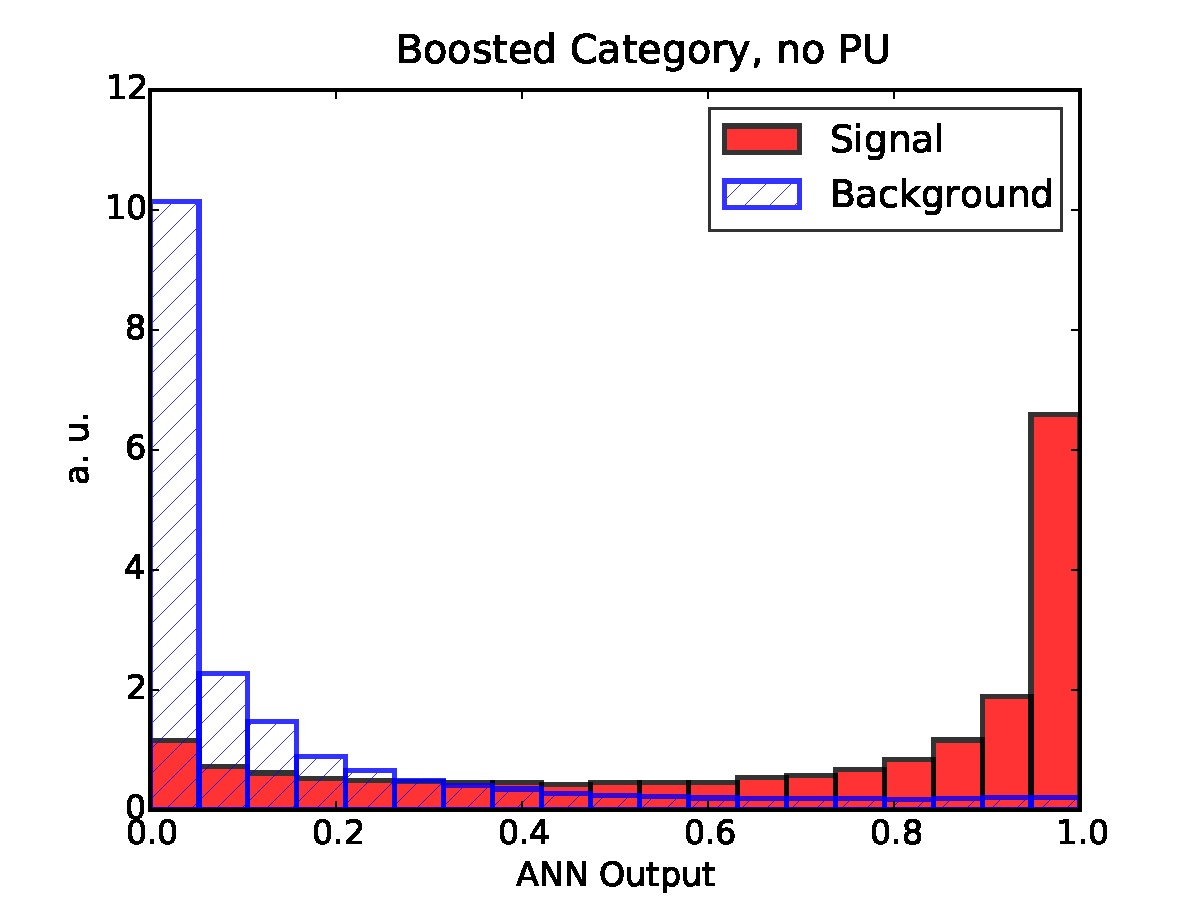
\includegraphics[width=0.65\textwidth]{plots/Boosted_disc_noPU.pdf}
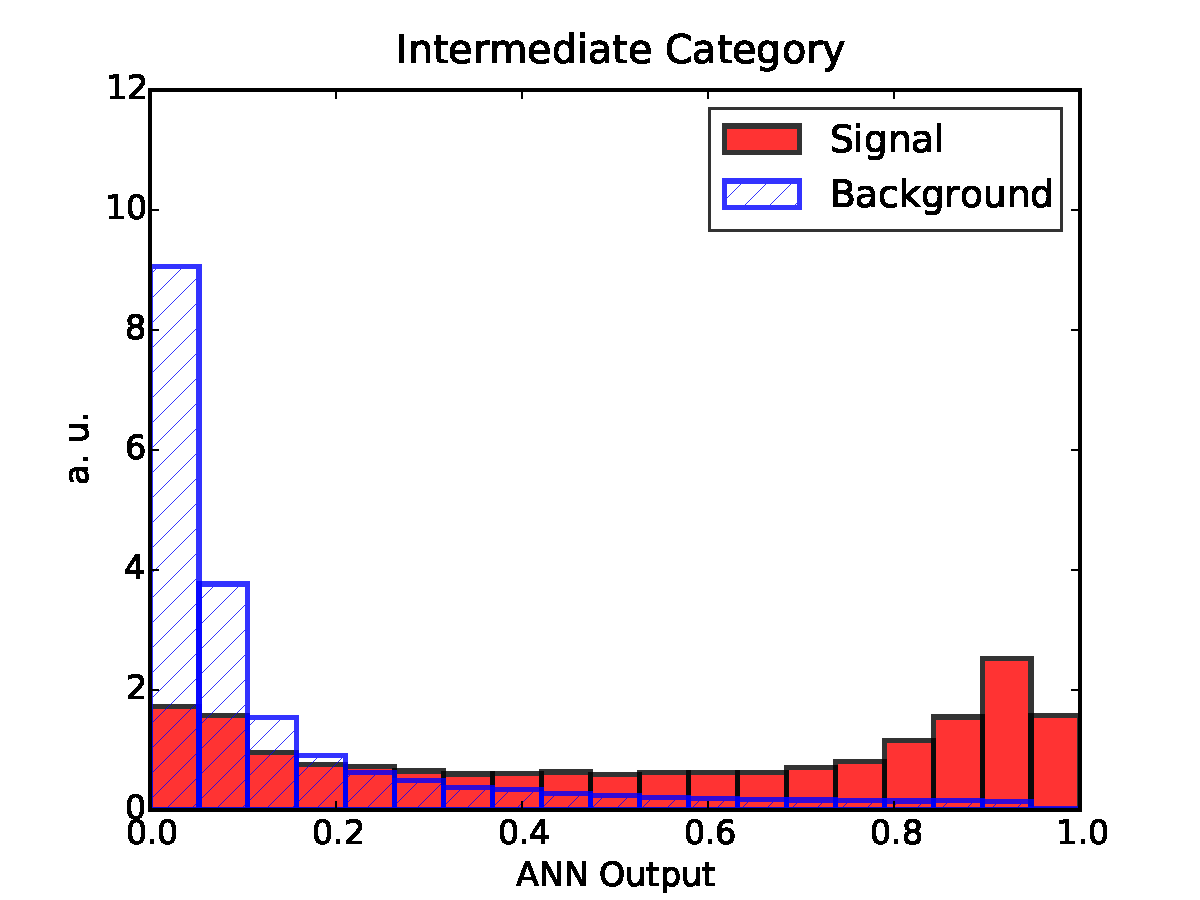
\includegraphics[width=0.48\textwidth]{plots/Intermediate_disc_noPU.pdf}
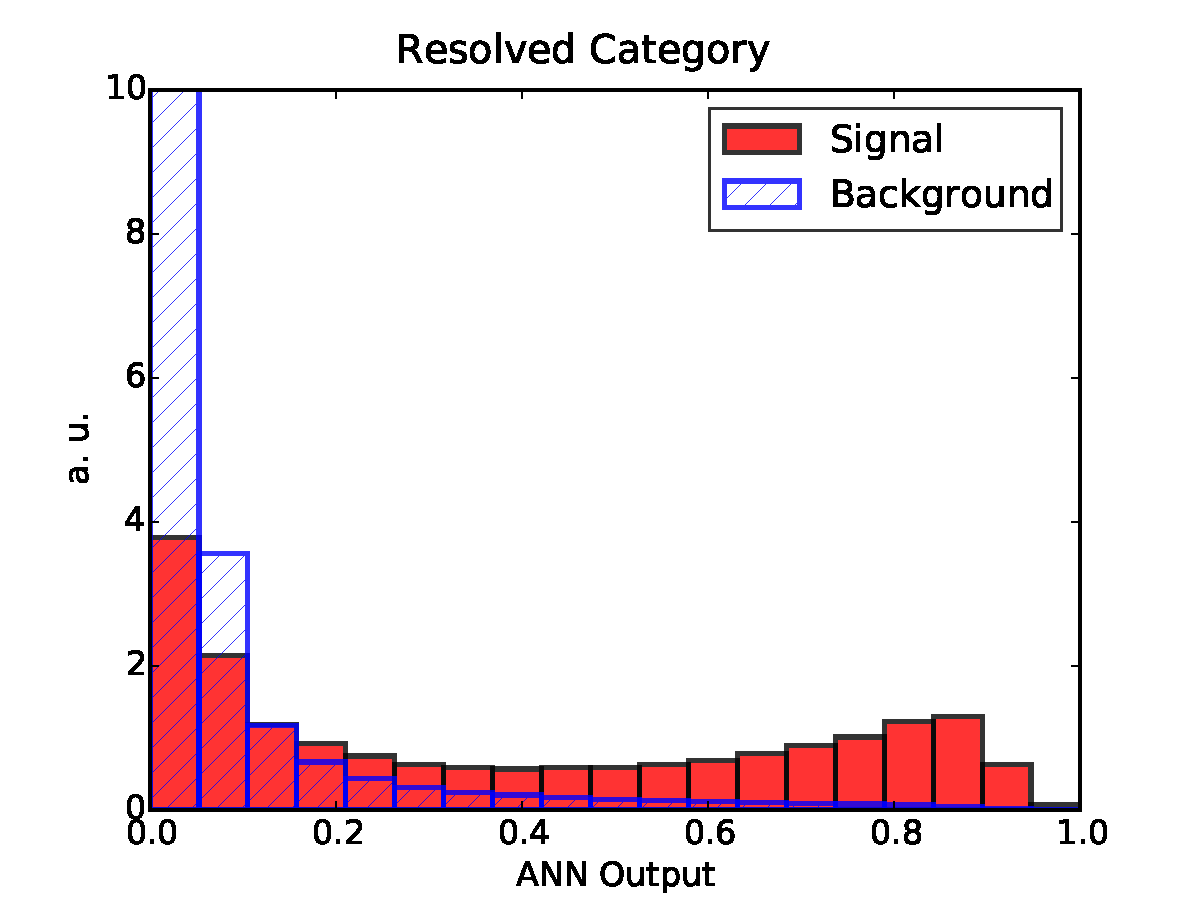
\includegraphics[width=0.48\textwidth]{plots/Resolved_disc_noPU.pdf}
\caption{\small The distribution as a function of the ANN output
  for the signal and background MC events in the three categories:
  boosted (upper plot), intermediate (lower left plot) and
  resolved (lower right plot).
  %
  All distributions are normalized so that their integral
  adds up to one.
}
\label{fig:nnresponse}
\end{center}
\end{figure}
%%%%%%%%%%%%%%%%%%%%%%%

From Fig.~\ref{fig:nnresponse} we see that in the boosted category the MVA manages
to achieve a clear discrimination between signal and background, with the two distributions
nicely peaking at 1 and at 0 respectively.
%
This indicates that introducing a suitable cut
$y_{\rm cut}$
in the ANN output will substantially reduce the background,
while keeping a reasonable signal efficiency.
%
The performance of the MVA discrimination is similar though slightly worse in the intermediate
category, and it is markedly worse in the resolved category.
%
We have traced back these differences to the use of jet substructure variables
in the boosted and intermediate categories, whose use substantially
improves the
discrimination between signal and background events.



The results for the signal selection efficiency and the 
background rejection rate as a function of the cut in the ANN output
$y_{\rm cut}$
define the so-called  Receiver-Operating Characteristic (ROC)
curve.
%
It is clear that we can achieve  high signal efficiency by using
a small value of the cut in the ANN output, but this choice will be
affected from a poor background
rejection.
%
Conversely, using a higher value of the cut will increase background rejection at the
cost of dropping signal efficiency.
%
The usefulness of ROC curves is that they allow to determine and
optimal cut value that removes enough background without degrading too much the signal efficiency.
%
Another important requirement on the value of $y_{\rm cut}$ is that
the  number of expected  signal events (the physical
events for a given integrated
luminosity, not the MC events used for the ANN training)
after the cut is large enough.


In Fig.~\ref{fig:exampleroc} the
we show the ROC curve for the background rejection rate as a function of the signal
  selection efficiency as the cut in the ANN output is varied.
  %
  We show the results for the three exclusive categories: boosted, intermediate
  and resolved.
%
As could already be inferred from the distribution of neural
networks output in Fig.~\ref{fig:nnresponse}, we find
that the neural network MVA is reasonably efficient
in discriminating signal over background.
%
The performance is best in the case of the boosted category,
decreasing then for the intermediate and finally for the
resolved categories, consistent with the distributions in
Fig.~\ref{fig:exampleroc}.
%



%%%%%%%%%%%%%%%%%%%%%%%%%%%%%%%%%%%%%%%%%%%%%%
\begin{figure}[t]
\begin{center}
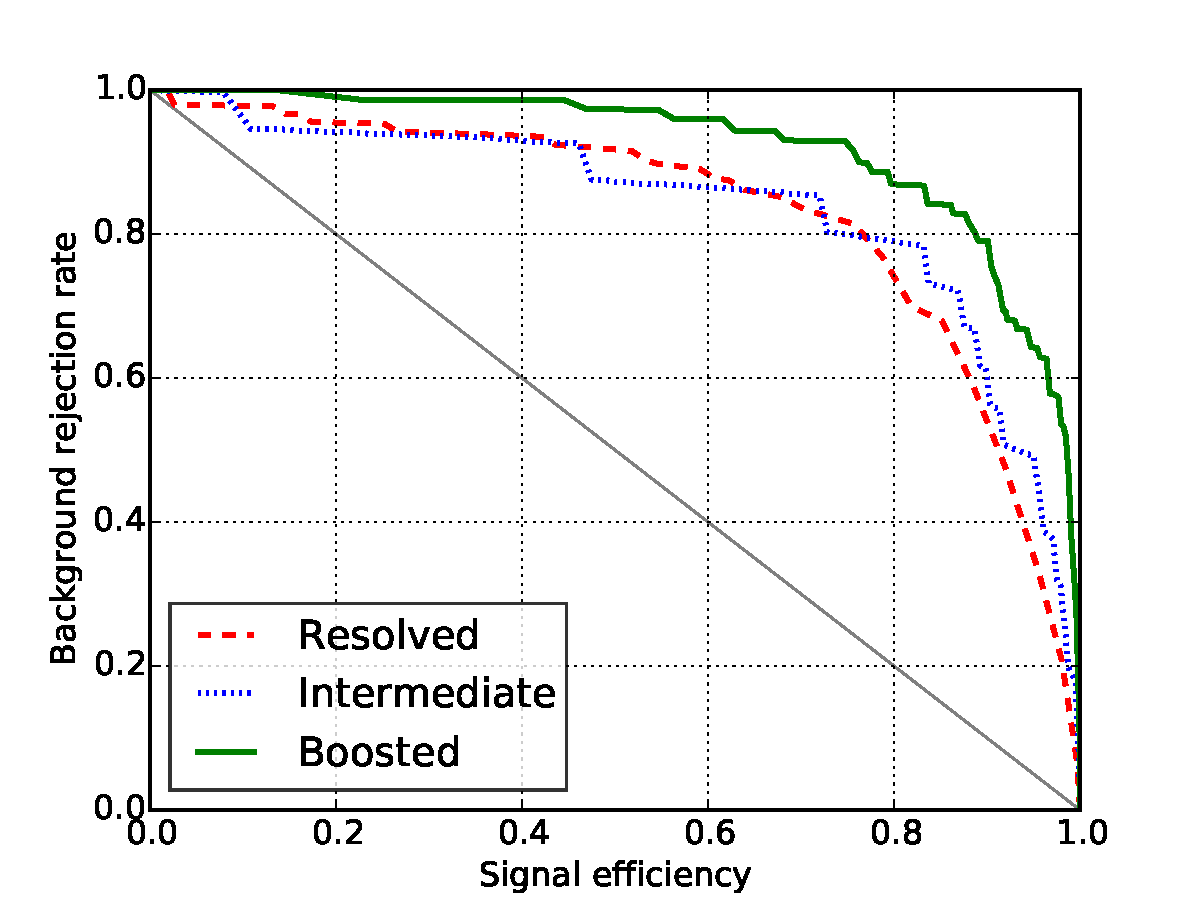
\includegraphics[width=0.65\textwidth]{plots/roc.pdf}
\caption{\small ROC curve for the background rejection rate as a function of the signal
  selection efficiency, as the cut in the ANN output is varied.
  %
  We show the results for the three exclusive categories: boosted, intermediate
  and resolved.
}
\label{fig:exampleroc}
\end{center}
\end{figure}
%%%%%%%%%%%%%%%%%%%%%%%%%%%%%%%%%%%%%

From Fig.~\ref{fig:exampleroc} we see that, always starting from the signal
and background events that survive the basic cut-based analysis,
one can achieve a  signal
efficiency of $\sim 90\%$ while reducing the background by
$80\%$, $60\%$ and $50\%$ in the boosted, intermediate and resolved
categories respectively.
%
It is easy to translate these factors into an  improvement factor of the pre-MVA
signal significance $S/\sqrt{B}$.
%
As an illustration, if a signal efficiency of 90\%
is required, we find that the MVA improves $S/\sqrt{B}$
by  approximately 2.0, 1.4 and 1.3  in the three categories respectively.

As mentioned above, an
 important restriction on the range of allowed cuts in the ANN output
 is that $y_{\rm cut}$
 cannot be so hard that the actual number of signal events expected
at the HL-LHC becomes unreasonably small.
%
To verify how many signal and background events are left after the MVA cut,
we show in Fig.~\ref{fig:nev2} the number of signal (dashed lines) and background (solid lines)
  events expected at the HL-LHC as a function of $y_{\rm cut}$,
  for the three exclusive categories.
  %
  Note that the value of the cut in the ANN cut is separately optimised in the three
  categories.

%%%%%%%%%%%%%%%%%%%%%%%%%%%%%%%%%%%%%%%%%%%%%%
\begin{figure}[t]
\begin{center}
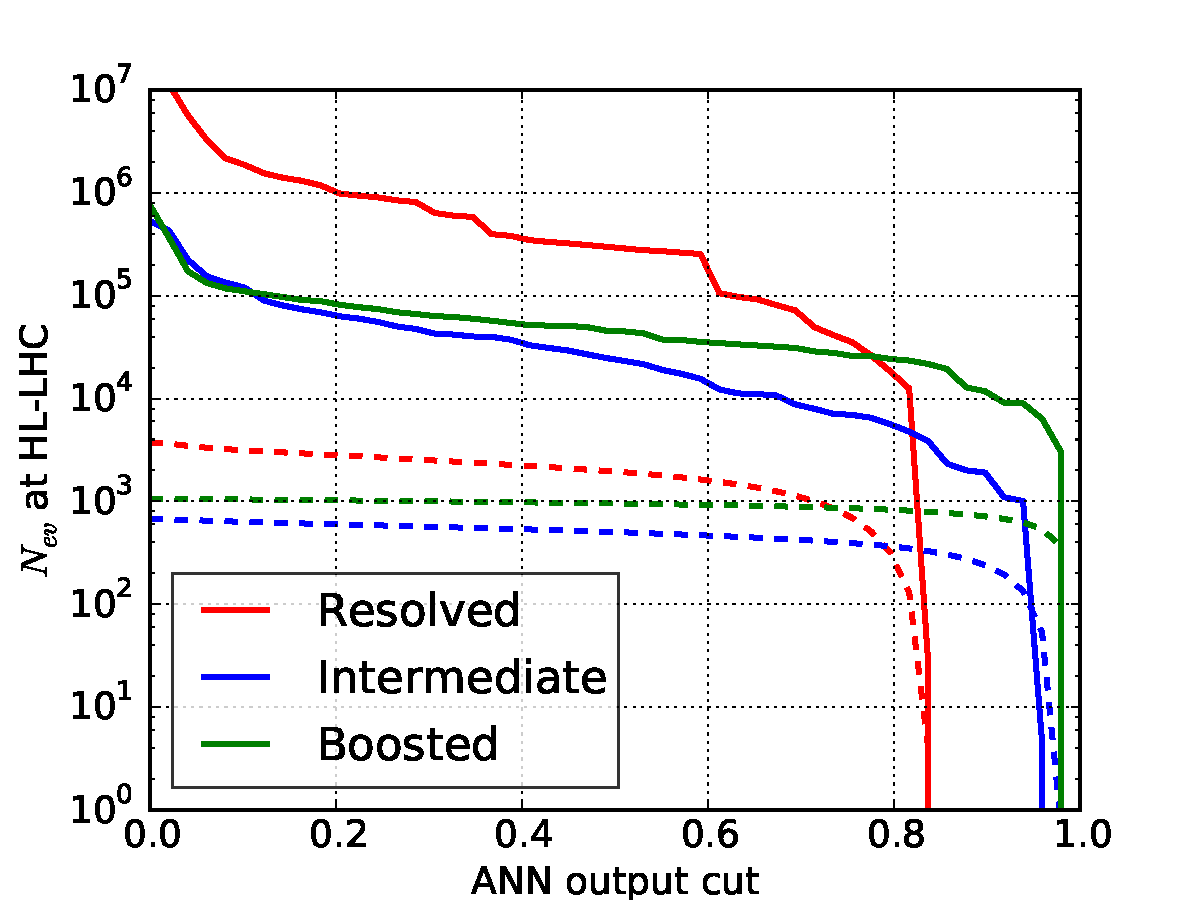
\includegraphics[width=0.65\textwidth]{plots/nev2_noPU.pdf}
\caption{\small Number of signal (dashed lines) and background (solid lines)
  events expected at the HL-LHC as a function of the cut in the ANN output,
  for the three separate categories.
}
\label{fig:nev2}
\end{center}
\end{figure}
%%%%%%%%%%%%%%%%%%%%%%%%%%%%%%%%%%%%%

As can be seen from Fig.~\ref{fig:nev2}, in the boosted category
event with a cut in the ANN output as hard as $y_{\rm cut}\simeq 0.9$
we are still left
with around 100 events at the HL-LHC, which is a reasonable number,
which the background being reduced substantially to around
1000 events.
%
A similar cut would work fine for the intermediate category, though here
the backgrounds are much larger and thus the expected signal significance smaller.
%
For the resolved case, the signal significance would be only slightly
improved for any value of the cut.

A useful property of MVAs such as the one used in this work
is that they provide direct  physical insight about which of the
input variables contribute the most to the separation of
signal over background.
%
In the case of ANNs, this can be quantified by computing the sum
of the absolute value of al the weights connected to a given
input neuron $i$, that is
\be
\label{eq:totweight}
\omega^{\rm tot}_i \equiv \sum_{k=1}^{n^{(2)}} \Big|\omega^{(2)}_{ki}\Big| \, ,
\qquad i=1,\ldots,N_{\rm var} \, ,
\ee
with $\omega^{(2)}_{ki}$ the value of the weight connecting
the $k$-th neutron of the second layer with the $i$-th neuron of
the first (input) layer, and $n^{(2)}=5$ the number of
neurons in the second layer.
%
The input variables with a larger value of $\omega^{\rm tot}_i$ will those
be the ones that play a dominant role in enhancing the signal
discrimination using the MVA.

%
In Fig.~\ref{fig:nnweights} we show
the distribution of the total associated weight,
Eq.~(\ref{eq:totweight}) for each of the $N_{\rm var}$ input
variables of the resolved (left plot) and boosted (right plot) categories.
%
The notation for the various kinematic variables is the same
as in Sect.~\ref{sec:input}.
%
The important information
is contained in the relative strengths of the total associated weight
for each of the input variables.
%
The results of Fig.~\ref{fig:nnweights} illustrate which variables
are more discriminative between the signal and the background.
%
For instance, in the 
resolved category, the variables that lead to
a higher discrimination power
are the $p_T$ of the two reconstructed Higgs candidates, and then on a similar
footing other variables like the $p_T$ of the individual jets
and the mass of the di-Higgs system $m_{hh}$.
%
The only variable which seems to contain to information at all
is the $\Delta \phi_{hh}$ separation between the two
Higgs candidates.


%%%%%%%%%%%%%%%%%%%%%%%%
\begin{figure}[t]
\begin{center}
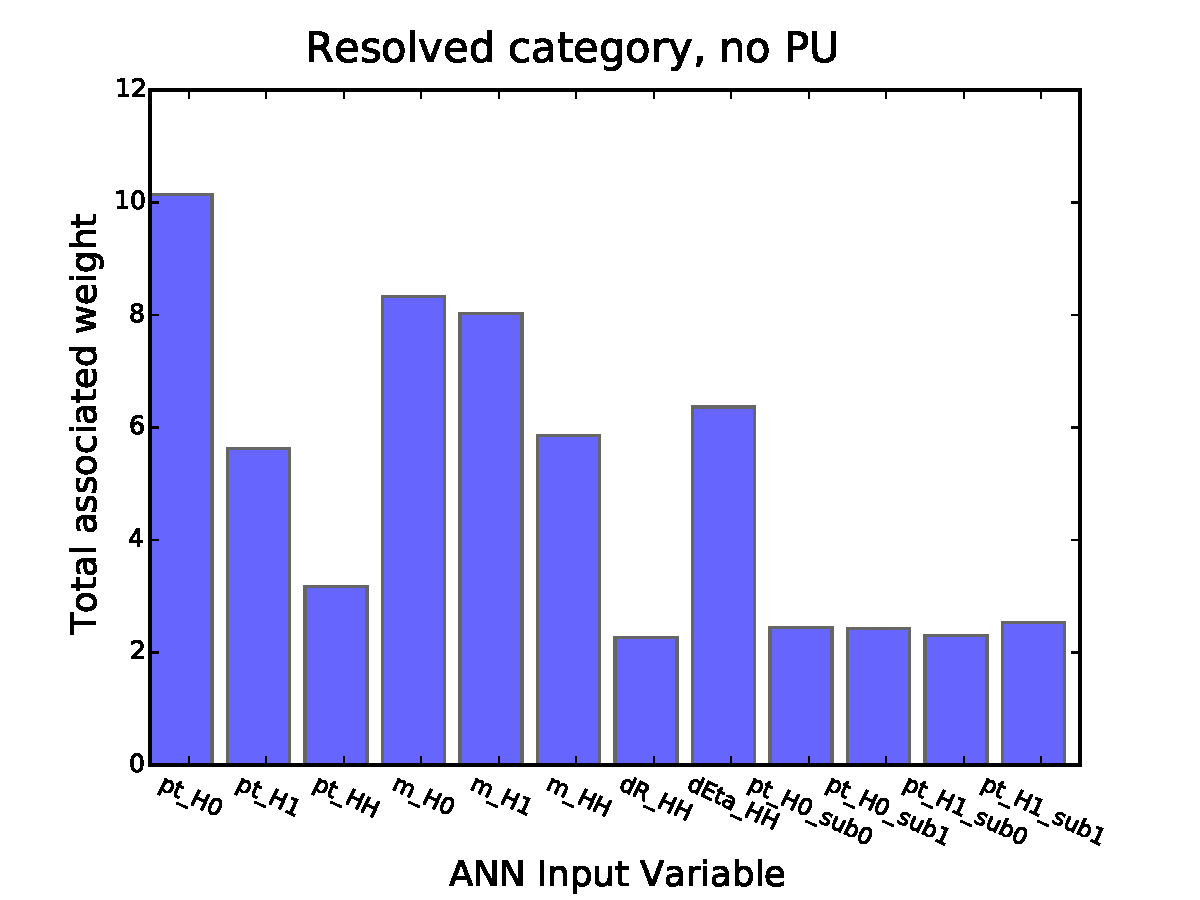
\includegraphics[width=0.49\textwidth]{plots/res_wgthist_noPU.pdf}
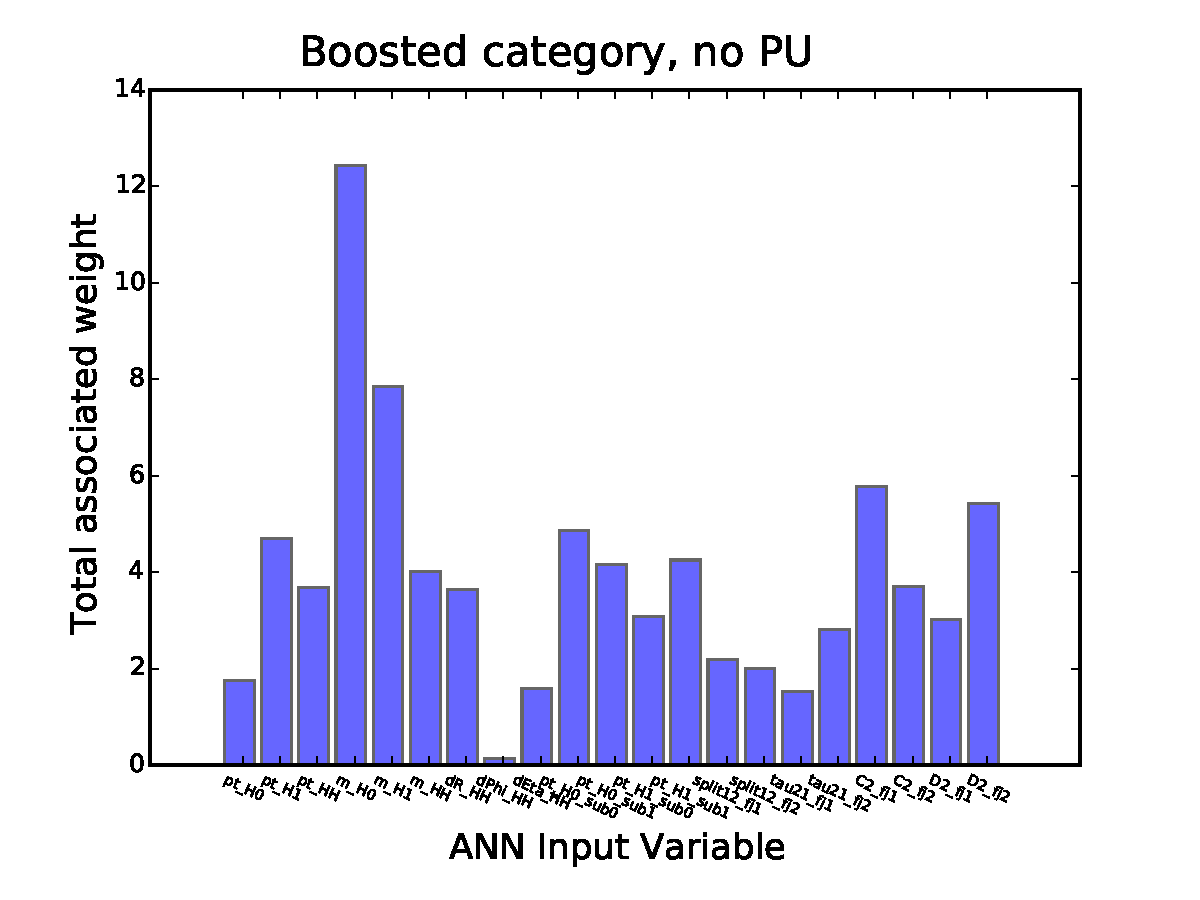
\includegraphics[width=0.49\textwidth]{plots/bst_wgthist_noPU.pdf}
\vspace{-0.5cm}
\caption{\small
Distribution of the total associated weight,
Eq.~(\ref{eq:totweight}) for each of the $N_{\rm var}$ input
variables of the resolved (left plot) and boosted (right plot) categories.
%
See Sect.~\ref{sec:input} for a description of each of the input
variables to the MVA.
}
\label{fig:nnweights}
\end{center}
\end{figure}
%%%%%%%%%%%%%%%%%%%%%%%




For the boosted category, we see that substructure variables
are the most helpful ones, in particular the $k_t$-splitting scale
$\sqrt{d_{12}}$ and the subjettiness ratio $\tau_{12}$.
%
The ratios of ECFs $D_2^{(\beta)}$ and
$C_2^{(\beta)}$ also seems to provide
useful discrimination power.
%
Concerning other kinematic variables, the angular
separation between the two large-$R$ jets $\Delta R_{hh}$,
the invariant mass of the di-Higgs system $m_{hh}$ and the various
$p_T$ also have discrimination power.
%
Other variables provide limited information, in particular the invariant
mass of the Higgs candidates, $m_{h_1}$ and $m_{h_2}$: this
is due to the realistic
simulation of detector resolution introduced with the smearing.
%
We have verified that the post-MVA
signal significance in the boosted category is substantially
degraded if substructure variables are not used.

At this point we have all the ingredients that we need to determine the optimal
value of the MVA output cuts $y_{\rm cut}$
and quantify the final values of the signal
significance $S/\sqrt{B}$ and $S/B$ in the three categories.
%
These optimal values are determined from the maximisation of $S/\sqrt{B}$,
ensuring that the number of events $N_{\rm ev}$
which would be expected at the HL-LHC is large
enough.
%
In addition, we also require when fixing $y_{\rm cut}$
that the actual number of MC events used for the ANN training
is large enough to avoid the biases of a small training sample.


The post-MVA results for $S/\sqrt{B}$ and $S/B$ as a function of the cut
in the ANN output for each of the three categories are shown in
Fig.~\ref{fig:sb_mva}.
%
Note that the values of $S/\sqrt{B}$ and $S/B$
for $y_{\rm cut}=0$ correspond to the values at
the end of the cut-based analysis, see
the {\bf C2} row of Table~\ref{table:cutflow}.
%
Indeed, at the end of the cut based analysis $S/\sqrt{B}$ was
approximately
1.0, 0.5 and 0.5 for the boosted, intermediate and resolved
categories, as can be seen from Fig.~\ref{fig:sb_mva}.
%
The same applies to $S/B$.

%%%%%%%%%%%%%%%%%%%%%%%%
\begin{figure}[t]
\begin{center}
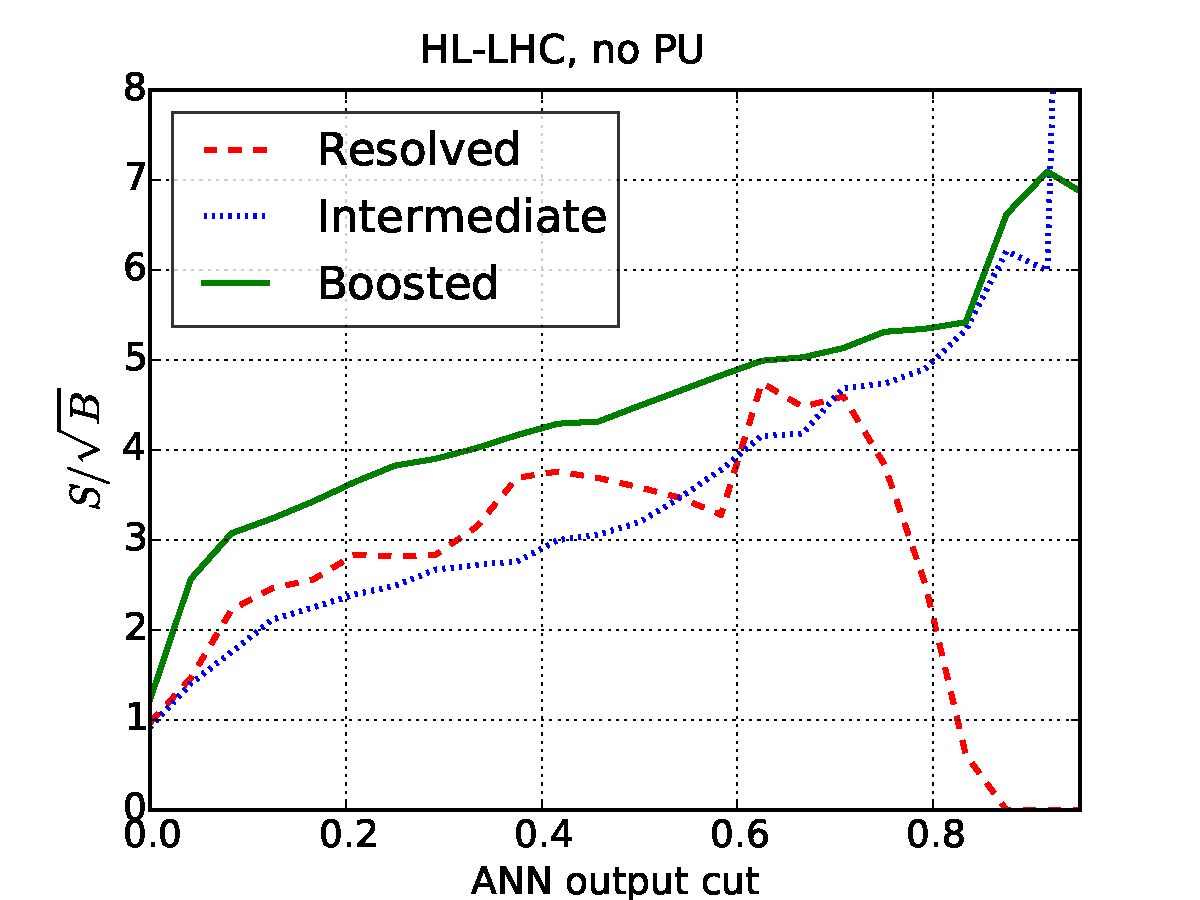
\includegraphics[width=0.48\textwidth]{plots/ssb_noPU.pdf}
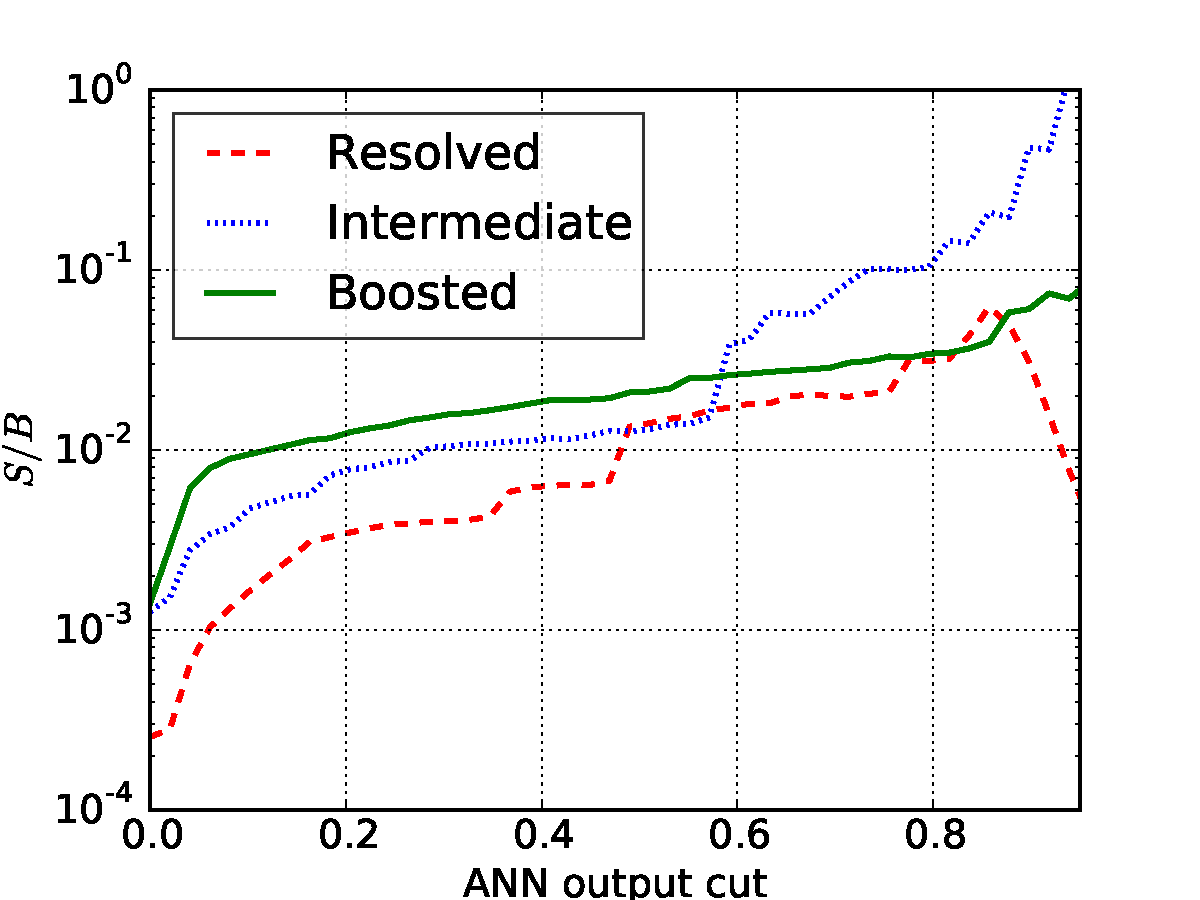
\includegraphics[width=0.48\textwidth]{plots/sb_noPU.pdf}
\caption{\small
  The values of the signal significance $S/\sqrt{B}$ and of the
  signal over background ratio $S/B$ for the boosted, intermediate
  and resolved categories as  function of the cut
  $y_{\rm cut}=0$ in the ANN output.
  %
  The $y_{\rm cut}=0$
  values correspond to the  cut-based analysis
  results from Table~\ref{table:cutflow}.
}
\label{fig:sb_mva}
\end{center}
\end{figure}
%%%%%%%%%%%%%%%%%%%%%%%

The results of Fig.~\ref{fig:sb_mva} are interesting in that they show
that for the resolved and boosted categories the improvement in signal
significance arising from the MVA is rather moderate, less that a factor two
in the two cases.
%
Even after the MVA, $S/\sqrt{B}$ never grows above 1.0.
%
The real power of the MVA can be seen for the boosted category,
where the signal significance rises from around 1.0 in the cut-based
analysis to above 3.0 for values of the ANN output cut $y_{\rm cut}\ge0.85$.
%
This value of the cut seems reasonable, since we know from Fig.~\ref{fig:nev2}
that the signal yield at the HL-LHC is still quite substantial,
of the order of 100 event.
%
Therefore, thanks to the MVA, we predict that one should be able
to find evidence for the production of Higgs boson pairs
at the HL-LHC using the $4b$ channel alone.

Another important benefit of the MVA applied to the boosted
category is that fact that the background is substantially
reduced so that $S/B$ can be as large as 10\% for the optimal
values of the ANN output cut.
%
Note that this is not true for the other two categories,
where $S/B$ is roughly constant.
%
A reasonably large value of $S/B$ is beneficial
from the experimental point of view, since it indicates
that the measurement is feasible even if the
systematic uncertainties are not very small.

Our final results are summarized in Table~\ref{table:cutflowMVA}, where we indicate
the value of the optimal ANN output
cut in each category,
the number of signal and background events $N_{\rm ev}$ expected
at the HL-LHC,
and also $S/\sqrt{B}$ and $S/B$.
%
For reference, we also include the results at the end of
the cut-based
analysis.
%



%%%%%%%%%%%%%%%%%%%%%%%%%%%%%%%%%%%%%%%%%%%%%%%%%%%%%
\begin{table}[t]
  \centering
  \begin{tabular}{c|c|c|c||c|c|c|c}
    \hline
    \multicolumn{8}{c}{Boosted category}\\
    \hline
    \hline
    \multicolumn{4}{c||}{no MVA cut} & \multicolumn{4}{c}{optimal MVA cut}\\
    \multicolumn{4}{c||}{$y_{\rm cut}=0$} & \multicolumn{4}{c}{$y_{\rm cut}=0.86$}\\
    \hline
    \multicolumn{2}{c|}{$N_{\rm ev}$} &  $S/\sqrt{B}$  & $S/B$
    & \multicolumn{2}{c|}{$N_{\rm ev}$} &  $S/\sqrt{B}$  & $S/B$\\
        Signal & Back   &     &   &  Signal & Back   &     &    \\
    \hline
      193   &  $3.8\,10^4$    &  0.99    &  $5.1\,10^{-3}$  & 107 & 1040 & 3.31  & 0.10\\
        \hline
  \end{tabular}
   $\,$\\
  \vspace{0.4cm}
  \noindent
  \begin{tabular}{c|c|c|c||c|c|c|c}
    \hline
    \multicolumn{8}{c}{Intermediate category}\\
    \hline
    \hline
    \multicolumn{4}{c||}{no MVA cut} & \multicolumn{4}{c}{optimal MVA cut}\\
    \multicolumn{4}{c||}{$y_{\rm cut}=0$} & \multicolumn{4}{c}{$y_{\rm cut}=0.49$}\\
    \hline
    \multicolumn{2}{c|}{$N_{\rm ev}$} &  $S/\sqrt{B}$  & $S/B$
    & \multicolumn{2}{c|}{$N_{\rm ev}$} &  $S/\sqrt{B}$  & $S/B$\\
        Signal & Back   &     &   &  Signal & Back   &     &    \\
    \hline
      660   &   $2.2\,10^6$   &   0.45   &  $3.1\,10^{-4}$ & 480  & $3.2\,10^5$ & 0.85  & $1.5\,10^{-3}$ \\
        \hline
  \end{tabular}
    $\,$\\
  \vspace{0.4cm}
  \noindent
  \begin{tabular}{c|c|c|c||c|c|c|c}
    \hline
    \multicolumn{8}{c}{Resolved category}\\
    \hline
    \hline
    \multicolumn{4}{c||}{no MVA cut} & \multicolumn{4}{c}{optimal MVA cut}\\
    \multicolumn{4}{c||}{$y_{\rm cut}=0$} & \multicolumn{4}{c}{$y_{\rm cut}=0.17$}\\
    \hline
    \multicolumn{2}{c|}{$N_{\rm ev}$} &  $S/\sqrt{B}$  & $S/B$
    & \multicolumn{2}{c|}{$N_{\rm ev}$} &  $S/\sqrt{B}$  & $S/B$\\
        Signal & Back   &     &   &  Signal & Back   &     &    \\
    \hline
    $1.6\,10^{3}$   &   $1.1\,10^{7}$   & 0.50     &  $1.5\,10^{-4}$   & 968 &
    $1.2\,10^{6}$  & 0.90 & $8.2\,10^{-4}$ \\
        \hline
  \end{tabular}
  \caption{\small The results for the number of signal and
    background events
    at the HL-LHC for both the cut-based analysis and after the
    optimal MVA cut, as well as the $S/\sqrt{B}$ and $S/B$
    values in the two cases.
    %
    From top to bottom we show the results for boosted,
    intermediate and resolved categories.
    %
    The value of the ANN output cut $y_{\rm cut}$
    is optimised separately in the
    three categories.
    \label{table:cutflowMVA}
  }
\end{table}
%%%%%%%%%%%%%%%%%%%%%%%%%%%%%%%%%%%%%%%%%%%%%%%%%%%%%

From Table~\ref{table:cutflowMVA} we see that after the
MVA the signal significance in the boosted category increases
from 0.99 to 3.31, with $S/B$ increasing from $0.005$ to $0.10$,
with still more that 100 signal events at the HL-LHC.
%
Table~\ref{table:cutflowMVA} also shows that for the intermediate
and resolved categories, the improvement due to the use
of the MVA is rather moderate, and signal significance is always
small since backgrounds are still  large.
%
The combination of the signal significance of the
three categories leads to a $S/\sqrt{B}=3.53$, and compared
to 3.31 using only the boosted category.


Table~\ref{fig:sb_mva} contains the main result of this paper:
at the HL-LHC, it should be possible to claim evidence of
Higgs pair production using only the $4b$ final state.
%
Needless to say, to claim discovery and to improve the accuracy
of the measurement of the trilinear coupling it would still
be needed to combine this channel with others like
$b\bar{b}\gamma\gamma$ and $b\bar{b}\tau\tau$, but in any case
it is always important to have robust evidence from
individual channels.

From Table~\ref{fig:sb_mva} it is also possible to
extract the signal significance that would be obtained
at the end of Run II with $\mathcal{L}_{\rm int}=300$ fb$^{-1}$:
in the boosted category we expect 11 signal events and 100 background
events, leading to a $S\sqrt{B}=1.1$, too small specially accounting
for realistic systematic experimental uncertainties.
%
So the full luminosity of the HL-LHC is really needed to exploit
the information contained in this final state, unless of course
new BSM dynamics enhance the di-Higgs production rates.

The results of Table~\ref{table:cutflowMVA} include
only the statistical uncertainty in the determination of
the background number of events.
%
We  briefly comment now how these results would be affected
if we also take into account the systematic experimental
uncertainty in the measurement
of the multijet backgrounds distributions.
%
While there is no unique definition of how signal significance is modified
by experimental systematic uncertainties~\cite{Bityukov:2002eq}, here we estimate
this effect with the simple correction
\be
\frac{S}{\sqrt{B}} \, \to \, \frac{S}{\sqrt{B}} \frac{1}{\sqrt{1+\lp \sigma^{\rm sys}\rp^2\cdot B}} \, ,
\ee
which corresponds to adding in quadrature to the statistical uncertainty  a single
uncorrelated systematic uncertainty $\sigma^{\rm sys}$.
%
Assuming an aggressive value of $\sigma^{\rm sys}=2\%$,
we find that the combined signal significance would be
reduced from 3.51 to 3.03.
%
While this quick estimate emphasizes the critical
importance of an experimentally accurate
measurement of multijet backgrounds at the LHC to fully exploit the $4b$
channel,
it is beyond the scope of this work to estimate realistically
the systematic uncertainties on QCD multijet distributions (and their bin-by-bin correlation)
that will be achieved at HL-LHC.


In the next section we discuss how the expectations for the HL-LHC
summarized in  Table~\ref{fig:sb_mva} are modified in different
conservative and aggressive scenarios for the performance of the
ATLAS and CMS experiments, in particular how the results depend
on the $b$-tagging performance and in the detector momentum
resolution.
%
But before that let us illustrate how the improvement in $S/\sqrt{B}$
obtained from the MVA in the boosted
category arises from the information contained in the
jet substructure variables.

\subsection{Another look at jet substructure variables}

%
From the distribution of total associated ANN weights in the
boosted category, shown in Fig.~\ref{fig:nnweights}, we see that
all substructure variables contain useful information:
the $k_t$-splitting scales $\sqrt{d_{12}}$,
the $\tau_{21}$ subjettiness ratio, and the ECF ratios
$C_2^{(\beta)}$ and $D_2^{(\beta)}$.
%
Interestingly, for some substructure variables, such as $\tau_{21}$,
the total associated weight turns out to be stronger in the leading
than in the sub-leading Higgs candidate (or vice-versa), indicating some
degree of redundancy when the same variable is used for the two Higgs candidates
at the same time.


The information reflected in Fig.~\ref{fig:nnweights} should also be
apparent from the corresponding distributions of these substructure
variables: those with a higher discrimination power should show
clear differences in shape between the signal and background events,
while those that carry less information should have similar
shapes for signal and background.
%
The third possibility is that of of redundant variables, where signal
and background exhibit different shapes but the same information
is already provided by other input variables.
%
To illustrate these points,
in Fig.~\ref{fig:mva_substructure_1}
we show the distributions of some of
these substructure variables for the boosted category: the
$k_t$ splitting scale $\sqrt{d_{12}}$, Eq.~(\ref{eq:ktsplitting}), for
the subleading Higgs,
the energy correlation double ratio $D_2^{(\beta)}$,
Eq.~(\ref{eq:d2}), for the leading Higgs,
and then 
the subjettiness ratio $\tau_{12}$,
Eq.~(\ref{eq:tau21}),
for both the leading and subleading Higgs candidates.
%

%%%%%%%%%%%%%%%%%%%%%%%%%%%%%%%%%%%%%%%%%%%%%%%%%%%%%%%
\begin{figure}[t]
  \begin{center}
    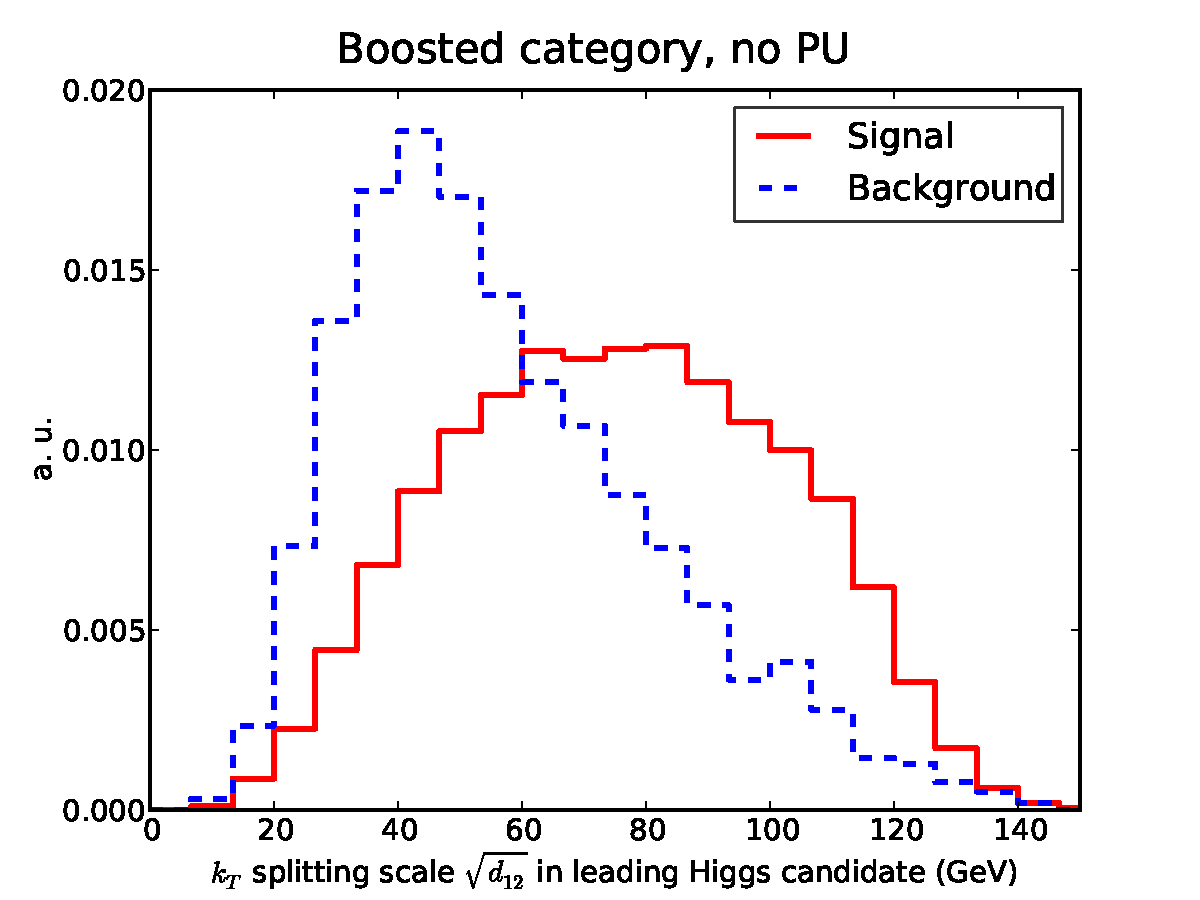
\includegraphics[width=0.48\textwidth]{plots/split12_h1_C1_boost.pdf} 
  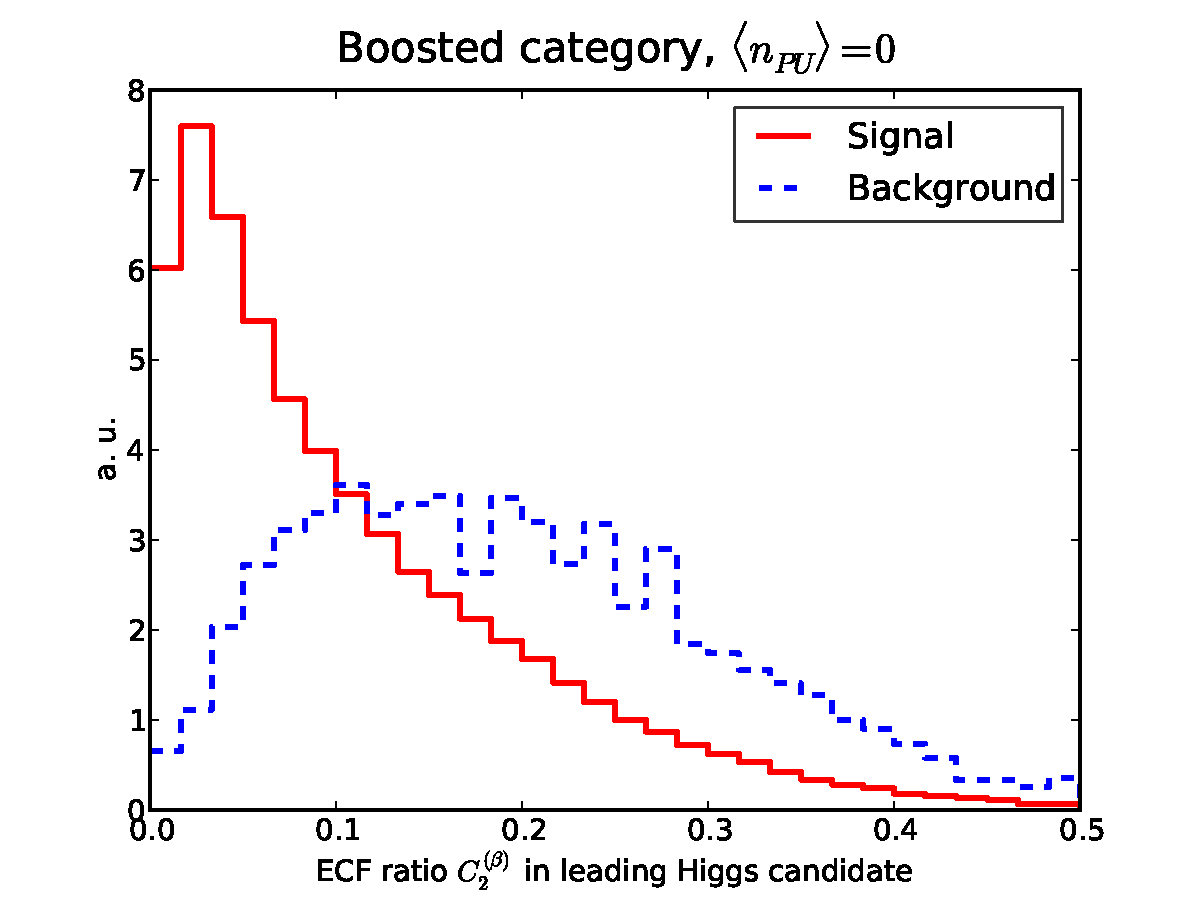
\includegraphics[width=0.48\textwidth]{plots/EEC_C2_h0_C1_boost.pdf}
  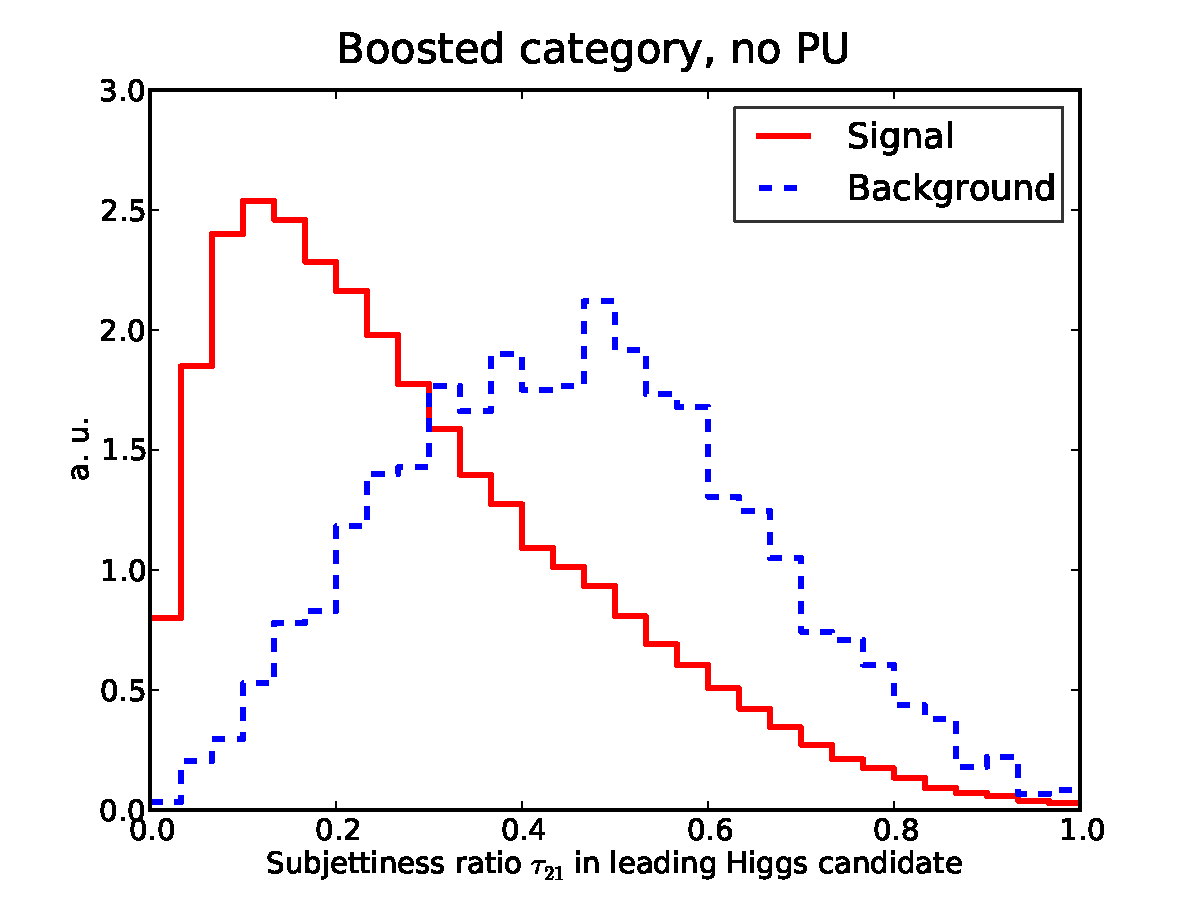
\includegraphics[width=0.48\textwidth]{plots/tau21_h0_C1_boost.pdf}
  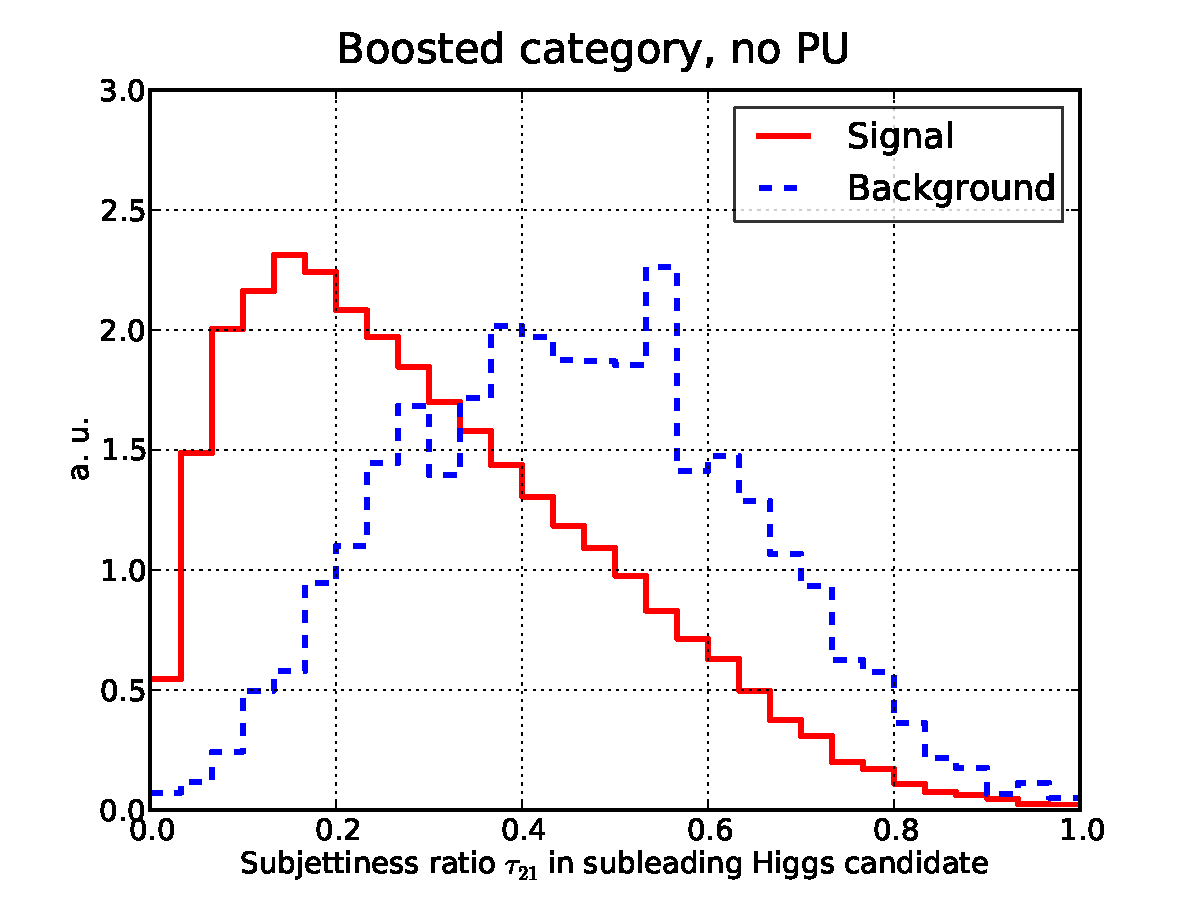
\includegraphics[width=0.48\textwidth]{plots/tau21_h1_C1_boost.pdf}
  \caption{\small Distribution of substructure variables
    in the boosted category at the end of the cut-based
    analysis, used as input to the MVA.
    %
    From top to bottom and from left to right we show  the
$k_t$ splitting scale for
the subleading Higgs, the subjettiness ratio $\tau_{12}$
for the leading Higgs,
and the energy correlation double ratio $D_2$
for the leading and subleading Higgs.
%
All distributions have been normalized to unity.
}
\label{fig:mva_substructure_1}
\end{center}
\end{figure}
%%%%%%%%%%%%%%%%%%%%%%%%%%%%%%%%%%%%%%%%%%%%%%%%%%%%%%%%%%%%%%%%%%%


From Fig.~\ref{fig:mva_substructure_1}
we can observe that for these substructure variables the shapes of the signal
and background distributions show important differences,
reflecting the inherent differences in the internal structure of jets
between QCD jets and jets originated from the Higgs decays.
%
Importantly, we observe that signal and background distributions peak
in different regions: for example, the $k_t$ splitting scale $\sqrt{d_{12}}$
peaks around 80 GeV (50 GeV) for signal (background) events, while
the ECF ratio $D_2^{(\beta)}$ peaks at much lower values for signal than
for background events.
%
From Fig.~\ref{fig:mva_substructure_1} we also see
the distributions of the subjettiness ratio $\tau_{12}$ are quite similar
in the leading and in the subleading jets, therefore adding
$\tau_{12}$ from the two Higgs candidates to the MVA at the same time
is redundant, explaining why in these cases either one or the other
variable from a Higgs candidate is assigned higher weight.


It is also interesting to show the distributions of kinematic variables
that according to the MVA provide a small amount of discrimination
between signal and background, and where the should not be an issue
of redundancy.
%
In Fig.~\ref{fig:mva_substructure_2}
we show the kinematic variable that carries less weight in the MVA,
    the azimuthal angle separation between the two Higgs candidates
    $\Delta\phi_{hh}$, for the resolved and boosted categories:
    according to Fig.~\ref{fig:nnweights}, essentially no discrimination power
    should be obtained from this variable, and indeed the shapes of the two signal
    and background
    are very similar here.
    %
    From Fig.~\ref{fig:nnweights} we also saw that the
    invariant mass distributions $m_h$ carry little information
    to discriminate signal over background:
    this was already verified from 
the corresponding
distributions in Fig.~\ref{fig:mHHinv}.
%
As explained before, the reduced discrimination power arises
from 
the  smearing of jet four-momenta introduced to mimic
realistically detector resolution.\footnote{We have verified that
  if no smearing is applied, the $m_h$ distributions for the leading
  and subleading Higgs candidates become the most
important variables in the MVA.}


%%%%%%%%%%%%%%%%%%%%%%%%%%%%%%%%%%%%%%%%%%%%%%%%%%%%%%%
\begin{figure}[t]
  \begin{center}
  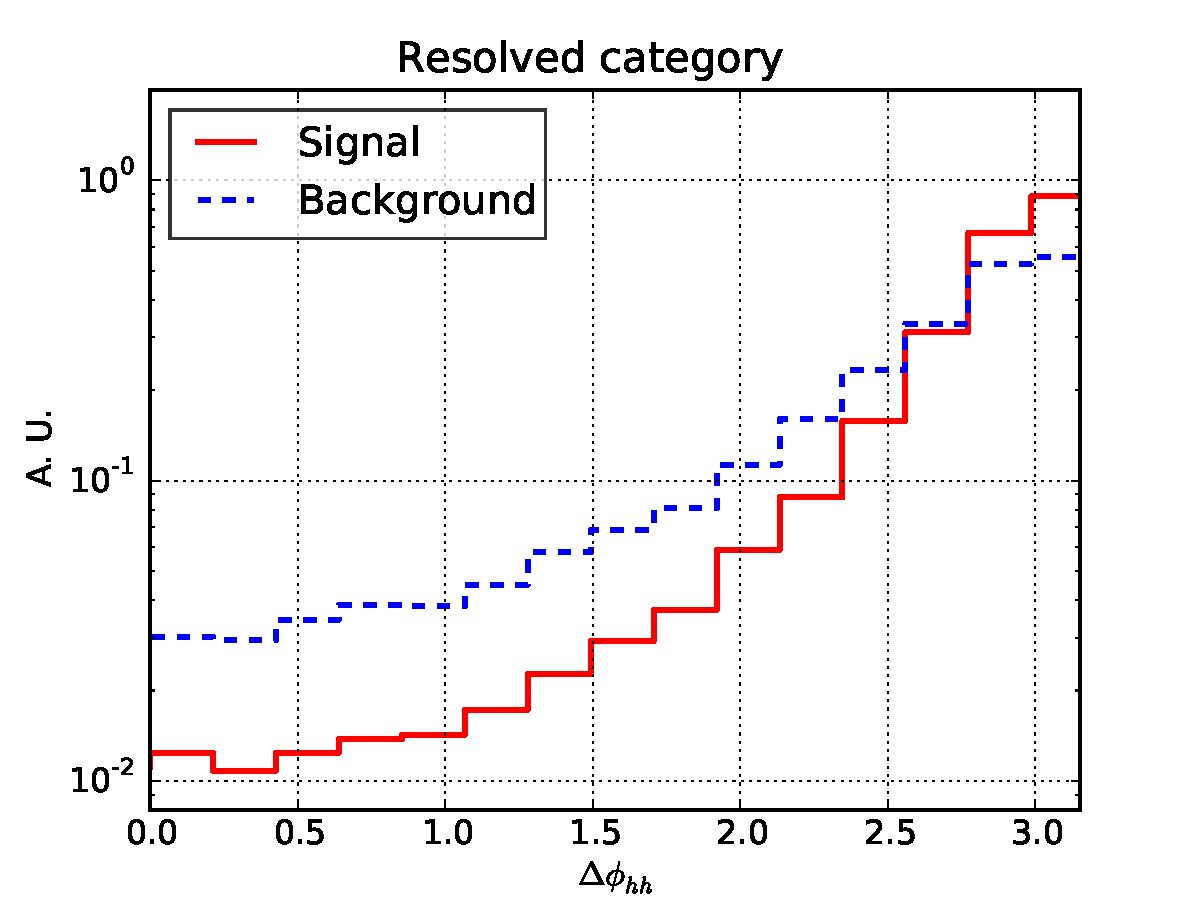
\includegraphics[width=0.48\textwidth]{plots/DeltaPhi_HH_C1_res.pdf} 
  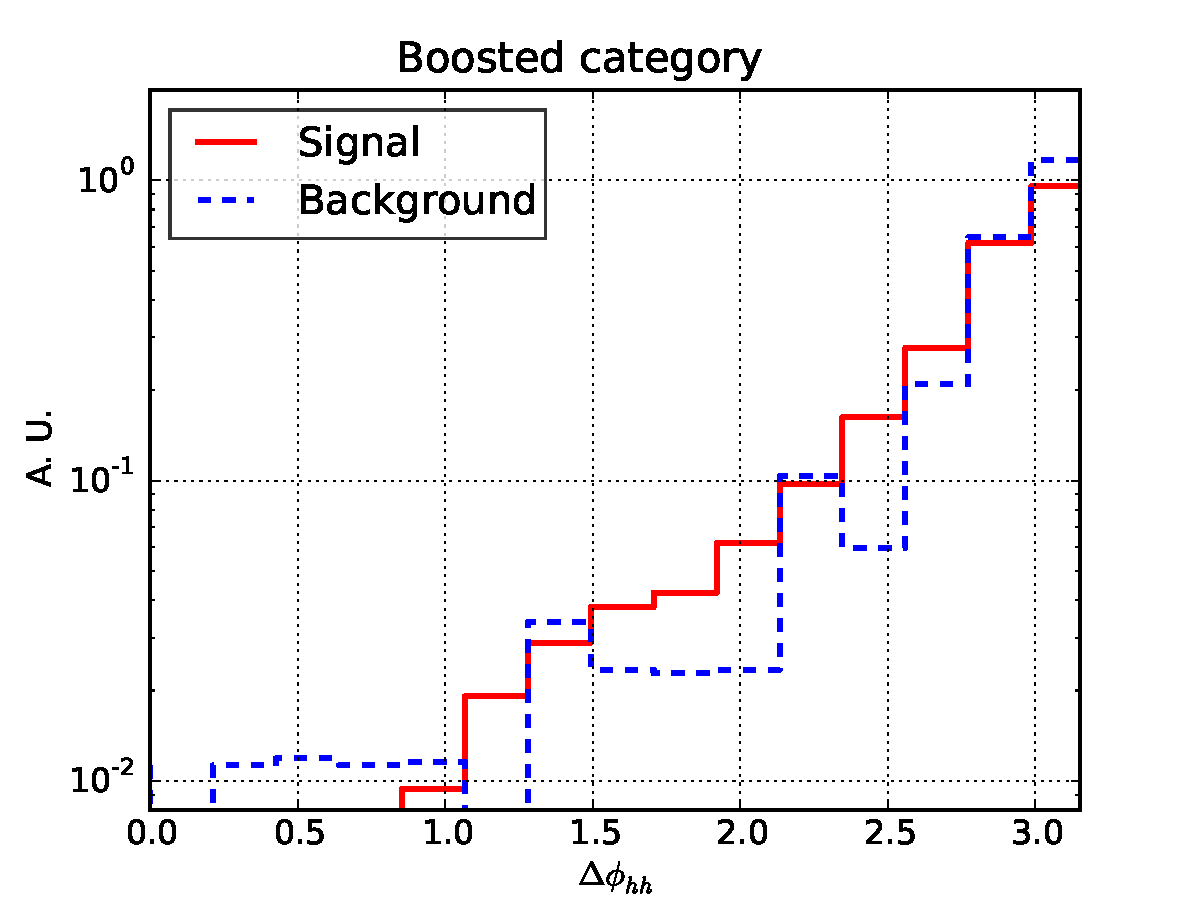
\includegraphics[width=0.48\textwidth]{plots/DeltaPhi_HH_C1_boosted.pdf} 
  \caption{\small Same as Fig.~\ref{fig:mva_substructure_1},
    now for the kinematic variable that carries less weight in the MVA,
    the azimuthal angle separation between the two Higgs candidates
    $\Delta\phi_{hh}$, for the resolved and boosted categories.
}
\label{fig:mva_substructure_2}
\end{center}
\end{figure}
%%%%%%%%%%%%%%%%%%%%%%%%%%%%%%%%%%%%%%%%%%%%%%%%%%%%%%%%%%%%%%%%%%%
